\documentclass[notes,11pt, aspectratio=169]{beamer}

\usepackage{pgfpages}
% These slides also contain speaker notes. You can print just the slides,
% just the notes, or both, depending on the setting below. Comment out the want
% you want.
\setbeameroption{hide notes} % Only slide
%\setbeameroption{show only notes} % Only notes
%\setbeameroption{show notes on second screen=right} % Both

\usepackage{helvet}
\usepackage[default]{lato}
\usepackage{array}
\usepackage{tgbonum}

\usepackage{tikz}
\usepackage{verbatim}
\setbeamertemplate{note page}{\pagecolor{yellow!5}\insertnote}
\usetikzlibrary{positioning}
\usetikzlibrary{snakes}
\usetikzlibrary{calc}
\usetikzlibrary{arrows}
\usetikzlibrary{decorations.markings}
\usetikzlibrary{shapes.misc}
\usetikzlibrary{matrix,shapes,arrows,fit,tikzmark}
\usepackage{amsmath}
\usepackage{mathpazo}
\usepackage{hyperref}
\usepackage{lipsum}
\usepackage{multimedia}
\usepackage{graphicx}
\usepackage{multirow}
\usepackage{graphicx}
\usepackage{dcolumn}
\usepackage{bbm}
\newcolumntype{d}[0]{D{.}{.}{5}}

\usepackage{changepage}
\usepackage{appendixnumberbeamer}
\newcommand{\beginbackup}{
   \newcounter{framenumbervorappendix}
   \setcounter{framenumbervorappendix}{\value{framenumber}}
   \setbeamertemplate{footline}
   {
     \leavevmode%
     \hline
     box{%
       \begin{beamercolorbox}[wd=\paperwidth,ht=2.25ex,dp=1ex,right]{footlinecolor}%
%         \insertframenumber  \hspace*{2ex} 
       \end{beamercolorbox}}%
     \vskip0pt%
   }
 }
\newcommand{\backupend}{
   \addtocounter{framenumbervorappendix}{-\value{framenumber}}
   \addtocounter{framenumber}{\value{framenumbervorappendix}} 
}


\usepackage{graphicx}
\usepackage[space]{grffile}
\usepackage{booktabs}
\newcommand\independent{\protect\mathpalette{\protect\independenT}{\perp}}
\def\independenT#1#2{\mathrel{\rlap{$#1#2$}\mkern2mu{#1#2}}}
\DeclareMathOperator{\Supp}{Supp}


\newtheorem{assN}{Assumption}
% These are my colors -- there are many like them, but these ones are mine.
\definecolor{blue}{RGB}{0,114,178}
\definecolor{red}{RGB}{213,94,0}
\definecolor{yellow}{RGB}{240,228,66}
\definecolor{green}{RGB}{0,158,115}

\hypersetup{
  colorlinks=false,
  linkbordercolor = {white},
  linkcolor = {blue}
}


%% I use a beige off white for my background
\definecolor{MyBackground}{RGB}{255,253,218}

%% Uncomment this if you want to change the background color to something else
%\setbeamercolor{background canvas}{bg=MyBackground}

%% Change the bg color to adjust your transition slide background color!
\newenvironment{transitionframe}{
  \setbeamercolor{background canvas}{bg=yellow}
  \begin{frame}}{
    \end{frame}
}

\setbeamercolor{frametitle}{fg=blue}
\setbeamercolor{title}{fg=black}
\setbeamertemplate{footline}[frame number]
\setbeamertemplate{navigation symbols}{} 
\setbeamertemplate{itemize items}{-}
\setbeamercolor{itemize item}{fg=blue}
\setbeamercolor{itemize subitem}{fg=blue}
\setbeamercolor{enumerate item}{fg=blue}
\setbeamercolor{enumerate subitem}{fg=blue}
\setbeamercolor{button}{bg=MyBackground,fg=blue,}



% If you like road maps, rather than having clutter at the top, have a roadmap show up at the end of each section 
% (and after your introduction)
% Uncomment this is if you want the roadmap!
% \AtBeginSection[]
% {
%    \begin{frame}
%        \frametitle{Roadmap of Talk}
%        \tableofcontents[currentsection]
%    \end{frame}
% }
\setbeamercolor{section in toc}{fg=blue}
\setbeamercolor{subsection in toc}{fg=red}
\setbeamersize{text margin left=1em,text margin right=1em} 

\newenvironment{wideitemize}{\itemize\addtolength{\itemsep}{10pt}}{\enditemize}

\usepackage{environ}
\NewEnviron{videoframe}[1]{
  \begin{frame}
    \vspace{-8pt}
    \begin{columns}[onlytextwidth, T] % align columns
      \begin{column}{.70\textwidth}
        \begin{minipage}[t][\textheight][t]
          {\dimexpr\textwidth}
          \vspace{8pt}
          \hspace{4pt} {\Large \sc \textcolor{blue}{#1}}
          \vspace{8pt}
          
          \BODY
        \end{minipage}
      \end{column}%
      \hfill%
      \begin{column}{.38\textwidth}
        \colorbox{green!20}{\begin{minipage}[t][1.2\textheight][t]
            {\dimexpr\textwidth}
            Face goes here
          \end{minipage}}
      \end{column}%
    \end{columns}
  \end{frame}
}

\title[]{\textcolor{blue}{Canonical Research Designs VII:\\ Regression
    Discontinuity I:\\ Identification and Groundwork}} \author[PGP]{}
\institute[FRBNY]{\small{\begin{tabular}{c}
                           Paul Goldsmith-Pinkham  \\
\end{tabular}}}

\date{\today}

\begin{document}

%%% TIKZ STUFF
\tikzset{   
        every picture/.style={remember picture,baseline},
        every node/.style={anchor=base,align=center,outer sep=1.5pt},
        every path/.style={thick},
        }
\newcommand\marktopleft[1]{%
    \tikz[overlay,remember picture] 
        \node (marker-#1-a) at (-.3em,.3em) {};%
}
\newcommand\markbottomright[2]{%
    \tikz[overlay,remember picture] 
        \node (marker-#1-b) at (0em,0em) {};%
}
\tikzstyle{every picture}+=[remember picture] 
\tikzstyle{mybox} =[draw=black, very thick, rectangle, inner sep=10pt, inner ysep=20pt]
\tikzstyle{fancytitle} =[draw=black,fill=red, text=white]
%%%% END TIKZ STUFF

% Title Slide
\begin{frame}
\maketitle
\end{frame}

\begin{frame}{Roadmap for Today}
  \begin{wideitemize}
  \item Today: regression discontinuity
  \item The goal will be to outline the simplest version of this
    approach, and how it works
  \item We will then discuss estimation in  straightforward
    settings
  \item Next class we will touch on more complicated settings and
    extensions
  \end{wideitemize}
\end{frame}

\begin{frame}{Regression Discontinuitiy}
    \begin{columns}[onlytextwidth, T] % align columns
      \begin{column}{.5\textwidth}
        \begin{wideitemize}
        \item Regression discontinuity has exploded onto the scene for empirical designs
        \item A rare case of a research design with random variation
          that is typically caused by real world constraints (and
          hence much more believable)
        \item Also the constraint is typically of interest directly
          \begin{itemize}
          \item The reduced form is interesting on its own, unlike
            some traditional IV papers
          \end{itemize}
        \item Also allows for \emph{graphical} presentation, a la
          binscatter, which creates transparency
        \end{wideitemize}
      \end{column}%
      \hfill%
      \begin{column}{.5\textwidth}
        \includegraphics[width=\linewidth]{images/rd_kleven_overtime.png}
      \end{column}%
    \end{columns}
\end{frame}

\begin{frame}{Examples}
    \begin{columns}[onlytextwidth, T] % align columns
      \begin{column}{.6\textwidth}
        \begin{wideitemize}
        \item The intellectual history of RD
          begins with Thistlewaite and Campbell (1960)
        \item But modern empirical examples begin with three notable examples:
          \begin{itemize}
          \item Van Der Klaauw (2002)
          \item Black (1999)            
          \item Angrist and Lavy (1999)
          \end{itemize}
        \item All on very different topics, but focused on discontinuous changes in some policy variables as a function of some smooth forcing variable:
          \begin{itemize}
          \item Educational scores
          \item Distance to border
          \item Class size
          \end{itemize}
        \end{wideitemize}
      \end{column}%
      \hfill%
      \begin{column}{.4\textwidth}
        \only<1>{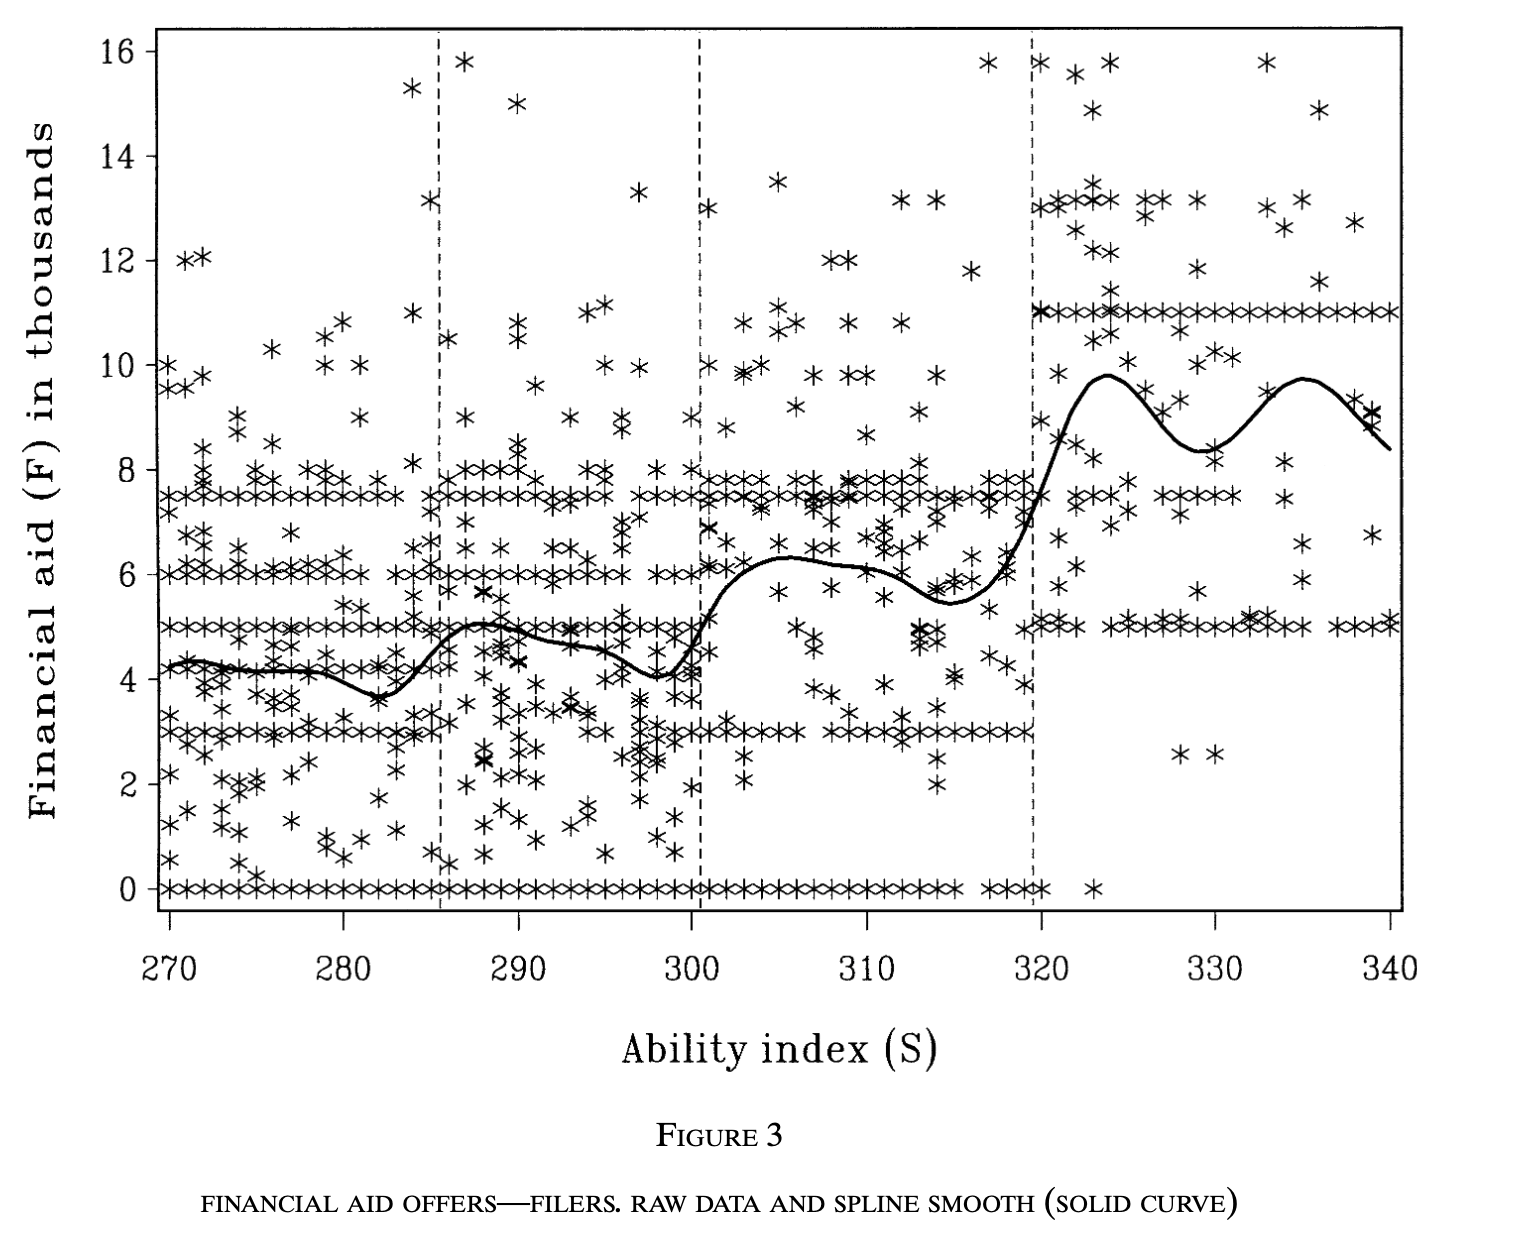
\includegraphics[width=\linewidth]{images/rd_ability.png}}
        \only<2>{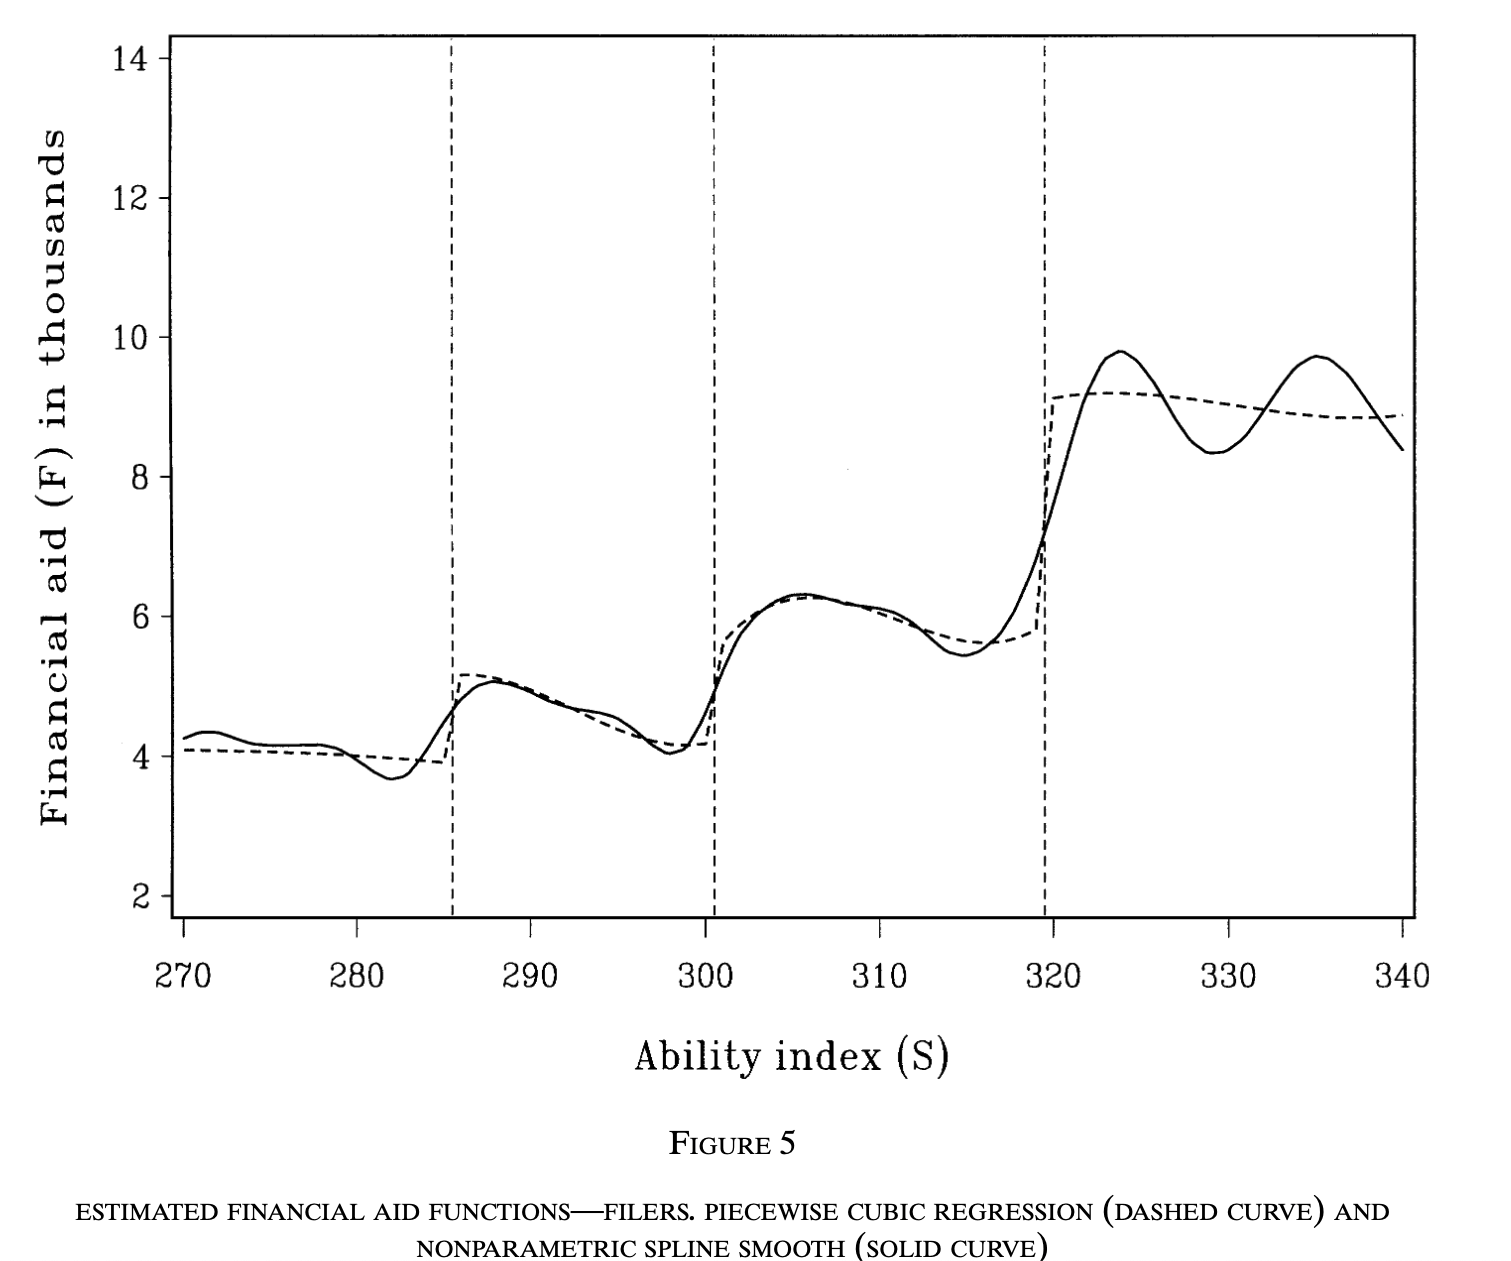
\includegraphics[width=\linewidth]{images/rd_ability3.png}}        
        \only<3>{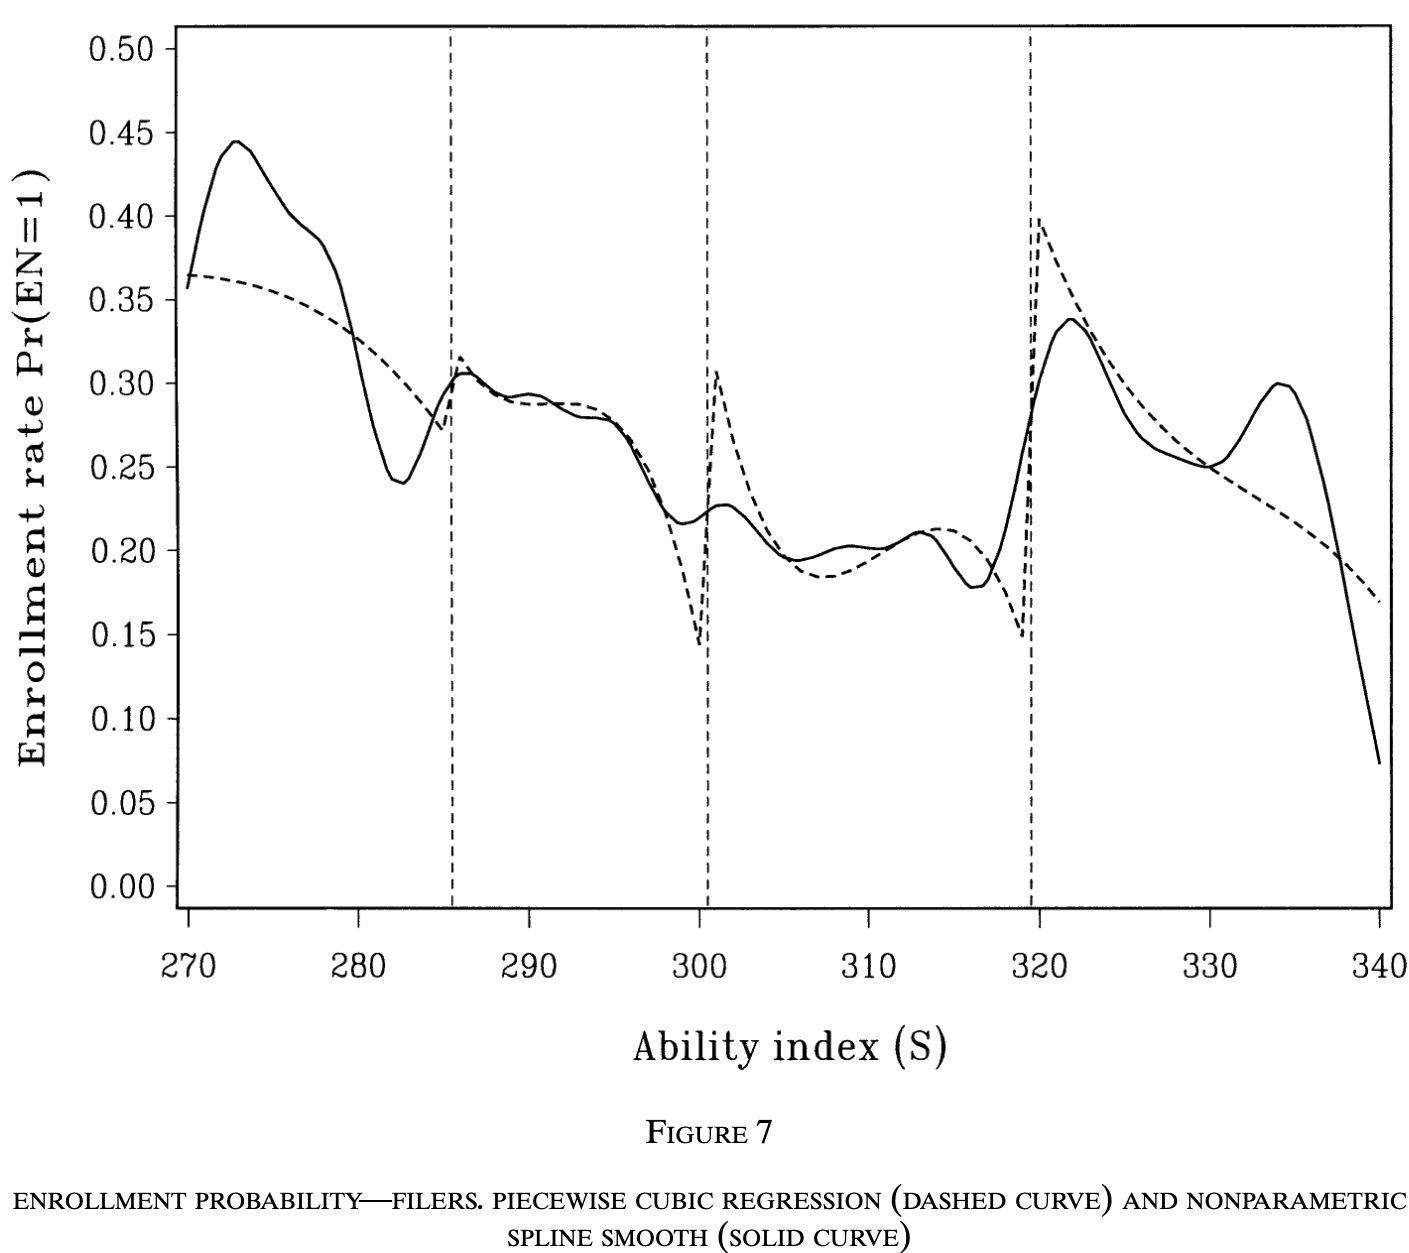
\includegraphics[width=\linewidth]{images/rd_ability2.png}}                
        \only<4>{\includegraphics[width=\linewidth]{images/rd_maimonides.png}}
      \end{column}%
    \end{columns}
\end{frame}

\begin{frame}{Notation for RD}
  \begin{columns}[onlytextwidth, T] % align columns
    \begin{column}{.8\textwidth}
      \begin{wideitemize}
      \item Setup notation first with traditional potential outcomes framework
        \begin{itemize}
        \item $Y_{i}(0)$, $Y_{i}(1)$, $D_{i} = \{0,1\}$, e.g. $Y_{i} = D_{i}Y_{i}(1) + (1-D_{i})Y_{i}(0)$
        \item Running variable: $Z_{i}$ (e.g. test score, distance or
          class size) -- normalize $Z_{i} = 0$ as the cutoff where the
          treatment $D_{i}$ is affected
      \end{itemize}
    \item Key parameter to focus on is the conditional mean $\mu_{Y}(z) = E(Y_{i} | Z_{i} = z)$
      \begin{itemize}
      \item Can think about more parts of distribution, but stronger requirement and will come to this later 
      \end{itemize}
    \item Need to distinguish between two cases:
      \begin{itemize}
      \item Sharp RD: at the cutoff, $D_{i} = 1$ vs. $D_{i} = 0$
      \item Fuzzy RD: at the cutoff, $E(D_{i}| Z_{i} = 0)$ changes
        discontinuously
        \begin{itemize}
        \item Fuzzy RD is just IV! We can consider a scaled version of
          our estimate that adjusts for the compliers shifted by the
          design
        \end{itemize}
      \end{itemize}
    \end{wideitemize}
  \end{column}%
  \hfill%
  \begin{column}{.4\textwidth}
    
  \end{column}%
\end{columns}
\end{frame}

\begin{frame}{What's the estimand? What's the goal?}
  \begin{wideitemize}
  \item Note that since $D_{i}$ discontinuously changes at
    $Z_{i} = 0$, if $E(Y_{i}|Z_{i})$ is sufficiently smooth, we can
    estimate the impact of $D_{i}$ on $Y_{i}$ at exactly $Z_{i} = 0$
    \begin{itemize}
    \item Key assumption: $E(Y_{i}(0) | Z_{i} = z)$ and
      $E(Y_{i}(1) | Z_{i} = z)$ are continuous in $z$
    \end{itemize}
  \item Under this assumption,  $\tau_{CATE} = E(Y_{i}(1) - Y_{i}(0) | Z_{i} = 0) = \lim_{z \downarrow 0}E(Y_{i} | Z_{i}= z) - \lim_{z \uparrow 0}E(Y_{i} | Z_{i}= z)$
    \begin{itemize}
    \item Note, this is a very particular subgroup of indiviudals, right at the cutoff
    \item Measure zero!
    \end{itemize}
  \item Next class, we'll discuss a design-based approach for thinking about this:
    \begin{itemize}
    \item More in line with our intuition that those around the cutoff
      are effectively ``randomly'' assigned
    \end{itemize}
  \item Note that this is no different than any non-parametric
    estimation problem that we've studied. Consider the ATE: $\tau_{ATT} = E(Y_{i}(1) - Y_{i}(0))$
    \begin{itemize}
    \item This estimand was estimated by needing an empirical analog
      for an unknowable $E(Y_{i}(1)$ and $E(Y_{i}(0))$
    \item With random assignment, we could estimate these.
      %$
    \item The complexity of RD arrives in estimation and inference
    \end{itemize}
  \end{wideitemize}
\end{frame}

\begin{frame}{Why is estimation harder for RD?}
  \begin{wideitemize}
    \item We need to estimate the counterfactual means at $Z_{i} = 0$
    \begin{itemize}
    \item We may not observe that point well, or at all
    \end{itemize}
  \item If $Z_{i}$ affects $Y_{i}$ (e.g. the running variable affects
    the outcome), then we need to both account for this running
    variable effect \emph{and} extrapolate
  \item Doing this in a flexible way asks substantially more of our data
    \begin{itemize}
    \item If we knew the parametric relationship between $Y$ and $Z$,
      this would be easy
    \end{itemize}
  \item Concretely, we need to understand how to estimate
    $\mu(z)$ at our cutoff variable
  \end{wideitemize}
\end{frame}

\begin{frame}{Aside on non-parametric estimation}
  \begin{wideitemize}
  \item What is non-parametric estimation? Model free approach to estimating features of the data
  \item In very simple cases, e.g. mean, variance, it is straightforward
    \begin{itemize}
    \item $\hat{E}(Y) = n^{-1}\sum_{i} Y_{i}$
    \end{itemize}
  \item However, you can consider non-parametric estimation for a wide range of problems
    \begin{itemize}
    \item The challenge becomes limitations in data
    \item Let's make this concrete
    \end{itemize}
  \end{wideitemize}
\end{frame}

\begin{frame}{Aside on non-parametric estimation}
%$
  \begin{columns}[onlytextwidth, T] % align columns
    \begin{column}{.8\textwidth}
      \begin{wideitemize}
      \item Consider the non-parametric estimation problem that you have
        likely tried and solved many times: density estimation
      \item This is the estimation of $\hat{f}(x)$ for a random variable $X_{i}$
        \begin{itemize}
        \item Note that in almost all cases when looking at densities, you
        consider scalar $X$ variable
        \end{itemize}
      \item Consider the case with a discrete variable $X_{i}$. In this case, estimation for $\hat{f}(x)$ is very straightforward:
        \begin{equation*}
          \hat{f}(x) = n^{-1}\sum_{i} 1(X_{i} = x)
        \end{equation*}
      \end{wideitemize}
    \end{column}%
    \hfill%
    \begin{column}{.4\textwidth}
    \end{column}%
  \end{columns}
\end{frame}

\begin{frame}{Aside on non-parametric estimation}
  \begin{columns}[onlytextwidth, T] % align columns
    \begin{column}{.6\textwidth}
      \begin{wideitemize}
      \item What if $X_{i}$ is continuous? The probability of $X_{i} =
        x$ is measure zero, so cannot just discretely bin
      \item The standard approach we learn is the histogram:
        \begin{equation*}
          \hat{f}(x) = (n_{k}/n) \times b, \; n_{k} = \sum_{i} 1(X_{i} \in \text{k interval}) 
        \end{equation*}
        and $b$ is the bin-width scaled by the range of the outcome
      \item Example from Lee (2008) running variable
      \end{wideitemize}
    \end{column}%
    \hfill%
    \begin{column}{.4\textwidth}
      \includegraphics[width=\linewidth]{images/lee_hist.png}
    \end{column}%
  \end{columns}
\end{frame}

\begin{frame}{Aside on non-parametric estimation}
  \begin{columns}[onlytextwidth, T] % align columns
    \begin{column}{.6\textwidth}
      \begin{wideitemize}
      \item   We can do better by using weights at each point in our dataset
      \item the histogram is bad because it is only ``right'' for certain
        points within the bin
        \begin{itemize}
        \item     (e.g. the approximation gets better and better as our bin size gets smaller)
        \end{itemize}
      \item   Clearly, the bandiwdth matters! What is the tradoeff?
        \begin{itemize}
        \item Bias vs. Variance! The larger the bandiwdth, the more
          precisely estimated, but more bias
        \item This issue comes up for RD as well
        \end{itemize}
      \end{wideitemize}
    \end{column}%
    \hfill%
    \begin{column}{.4\textwidth}
      \includegraphics[width=\linewidth]{images/lee_density.png}
    \end{column}%
  \end{columns}
\end{frame}

\begin{frame}{Aside on non-parametric estimation}
  \begin{columns}[onlytextwidth, T] % align columns
    \begin{column}{.7\textwidth}
  \begin{wideitemize}
  \item Formally, the density is estimated using kernel estimation as:
    \begin{equation*}
      \hat{f}(x) = \frac{1}{Nh}\sum_{i}K\left(\frac{X_{i} - c}{h}\right),
    \end{equation*}
    where $K$ denotes our \emph{kernel} weighting function
  \item Lots of things to know about kernels, but the key idea is that they sum to one.
    \begin{itemize}
    \item A histogram is just a uniform kernel weighting around a given point!
    \end{itemize}
  \item $h$ is our choice of bandwidth / smoothing parameter. The
    bigger the bandwidth, the wider your window
  \item Next class, we will discuss data-driven approaches for this
    \begin{itemize}
    \item However, limiting asymptotic argument requires that $h \to 0$
    \end{itemize}
  \end{wideitemize}
    \end{column}%
    \hfill%
    \begin{column}{.3\textwidth}
      \only<1>{\includegraphics[width=\linewidth]{images/lee_density_bw1.png}}
      \only<2>{\includegraphics[width=\linewidth]{images/lee_density_bw2.png}      }
    \end{column}%
  \end{columns}
\end{frame}


\begin{frame}{Challenges with non-parametric estimation}
  \begin{wideitemize}
  \item   Consider the problem of kernel estimation with two variables (or more)
  \item   The number of datapoints necessary grows exponentially with the
    dimension of the problem
  \item   This downside to non-parametrics becomes particularly clear once you
  consider non-parametric \emph{regression} 
  \end{wideitemize}
\end{frame}

\begin{frame}{Non-parametric regression}
  \begin{wideitemize}
  \item   Remember what we cared about what we started was $\mu(z) = E(Y| Z_{i} = z)$
  \item   Note what the expectation is:
  \begin{equation*}
    \mu(z) = \int y \; f(y | z) dy
  \end{equation*}
\item If $Z$ were discrete, this is a straightforward
  problem. However, once $Z$ is continuous, we need to smoothly draw
  on data from nearby points
\item This is the local regression approach (we will focus on the linear case)
  \begin{itemize}
  \item This exploits the fact that the function $\mu(z)$ is locally
    approximable by a linear function (as we get closer and closer --
    the same logic of a Taylor approximation)
  \end{itemize}
\item Hence, consider fitting the local regression around point $z$ with bandwidth $h$ with uniform kernel:
  \begin{equation}
    \min_{\alpha, \beta}\sum_{i | z-h < Z_{i} < z} (Y_{i} - \alpha - \beta (Z_{i} - z))^{2}
  \end{equation}
  \end{wideitemize}
\end{frame}


\begin{frame}{Aside on non-parametric estimation}
  \begin{wideitemize}
  \item More generally, consider the following general kernel problem:
    \begin{equation}
      \hat{\mu}(z) = \min_{\alpha, \beta}\sum_{i | z-h < Z_{i} < z} (Y_{i} - \alpha - \beta (Z_{i} - z))^{2} K_{h}(z - Z_{i})
    \end{equation}
    where $K_{h}(u) = h^{-1} K(u/h)$ is our kernel weight. Three examples worth knowing:
    \begin{itemize}
    \item Uniform: $K(u) = 0.5$ ($u$ runs from -1 to 1)
    \item Triangular: $K(u) = (1-|u|)$ ($u$ runs from -1 to 1)
    \item Epanechnikov: $K(u) = 0.75(1-u^{2})$ ($u$ runs from -1 to 1)    
    \end{itemize}
\item We now have all the tools we need to do RD!
  \begin{itemize}
  \item Recall that RD simply requires estimating $\mu_{z}$ at
    $z = 0$, using only data on the left, and only data on the right
  \end{itemize}
  \end{wideitemize}
  
\end{frame}

\begin{frame}{Checklist for estimation in RD}
  \begin{wideitemize}
  \item Choose kernel
    \begin{itemize}
    \item Uniform is really fine for RD -- if kernel matters, you likely have sensitive estimates
    \end{itemize}
  \item Choose bandwidth
    \begin{itemize}
    \item Can be done in a data-driven way
    \end{itemize}
  \item Estimate on left and right:
    \begin{itemize}
    \item $\tau_{SRD} = \lim_{z \downarrow 0} \mu(z) - \lim_{z \uparrow 0}  \mu(z)$
    \item And hence: $\hat{\tau}_{SRD} = \hat{\alpha}_{r} - \hat{\alpha}_{l}$ where
      \begin{align*}
        \hat{\alpha}_{l},\hat{\beta}_{l} &= \arg \min_{\alpha, \beta}\sum_{i | c-h < Z_{i} < c} (Y_{i} - \alpha - \beta (Z_{i} - c))^{2} K_{h}(c - Z_{i})\\
        \hat{\alpha}_{r},\hat{\beta}_{r}   &= \arg \min_{\alpha, \beta}\sum_{i | c < Z_{i} < c+h} (Y_{i} - \alpha - \beta (Z_{i} - c))^{2} K_{h}(c - Z_{i})\\
      \end{align*}
      
    \end{itemize}
  \end{wideitemize}
\end{frame}


\end{document}